%!TEX root = ../../paper.tex

\begin{figure*}
	\centering
	%!TEX root = ../../paper.tex

% Ferdosi 1 - MBE
\begin{subfigure}{0.3\textwidth}
	\centering
	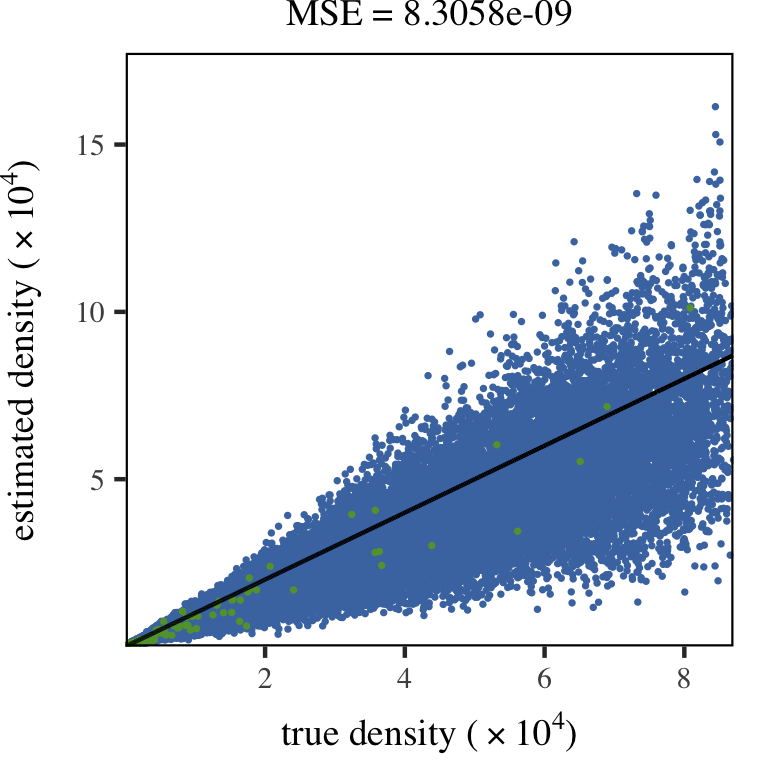
\includegraphics[keepaspectratio=true, width=\textwidth, height=0.23\textheight]{result/img/results_ferdosi_1_60000_mbe_silverman}
	\caption{Set \ferdosiOne, \mbe}
	\label{fig:results:singlesphere:mbe:ferdosi1}
\end{subfigure}
% Ferdosi 1 - SAMBE
\begin{subfigure}{0.3\textwidth}
	\centering
	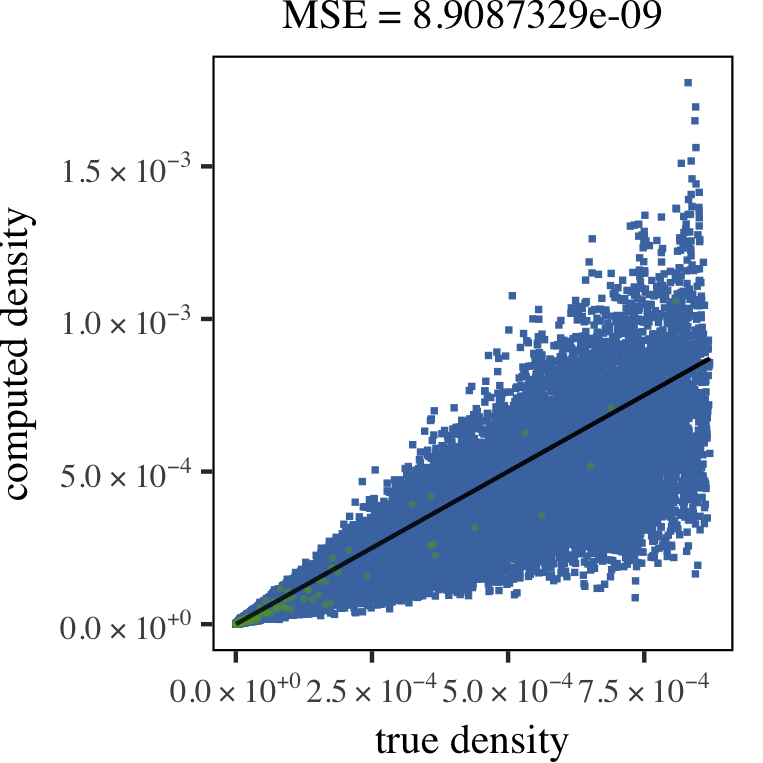
\includegraphics[keepaspectratio=true, width=\textwidth, height=0.23\textheight]{result/img/results_ferdosi_1_60000_sambe_silverman}
	\caption{Set \ferdosiOne, \sambe}
	\label{fig:results:singlesphere:sambe:ferdosi1}
\end{subfigure}
\subfigvspace
% Baakman 1	- MBE
\begin{subfigure}{0.3\textwidth}
	\centering
	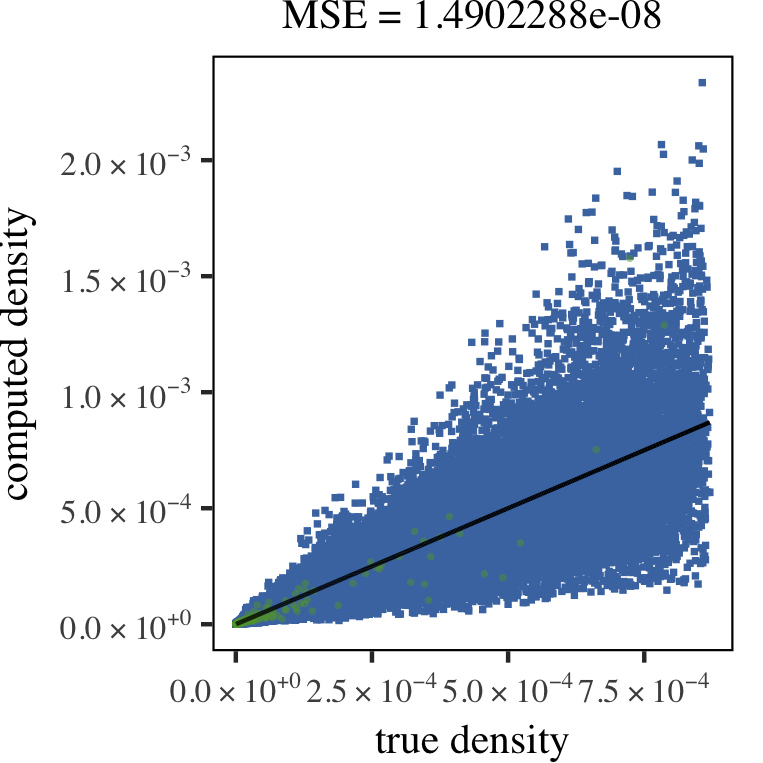
\includegraphics[keepaspectratio=true, width=\textwidth, height=0.23\textheight]{result/img/results_baakman_1_60000_mbe_silverman}
	\caption{Set \baakmanOne, \mbe}
	\label{fig:results:singlesphere:mbe:baakman1}
\end{subfigure}
% Baakman 1	- SAMBE
\begin{subfigure}{0.3\textwidth}
	\centering
	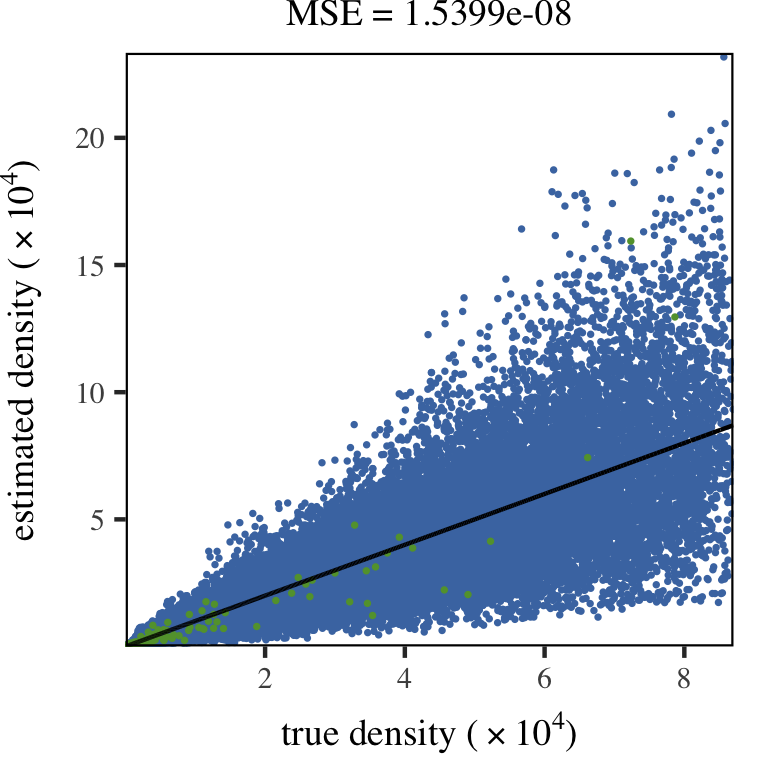
\includegraphics[keepaspectratio=true, width=\textwidth, height=0.23\textheight]{result/img/results_baakman_1_60000_sambe_silverman}
	\caption{Set \baakmanOne, \sambe}
	\label{fig:results:singlesphere:sambe:baakman1}
\end{subfigure}
\subfigvspace
% Baakman 4 - MBE
\begin{subfigure}{0.3\textwidth}
	\centering
	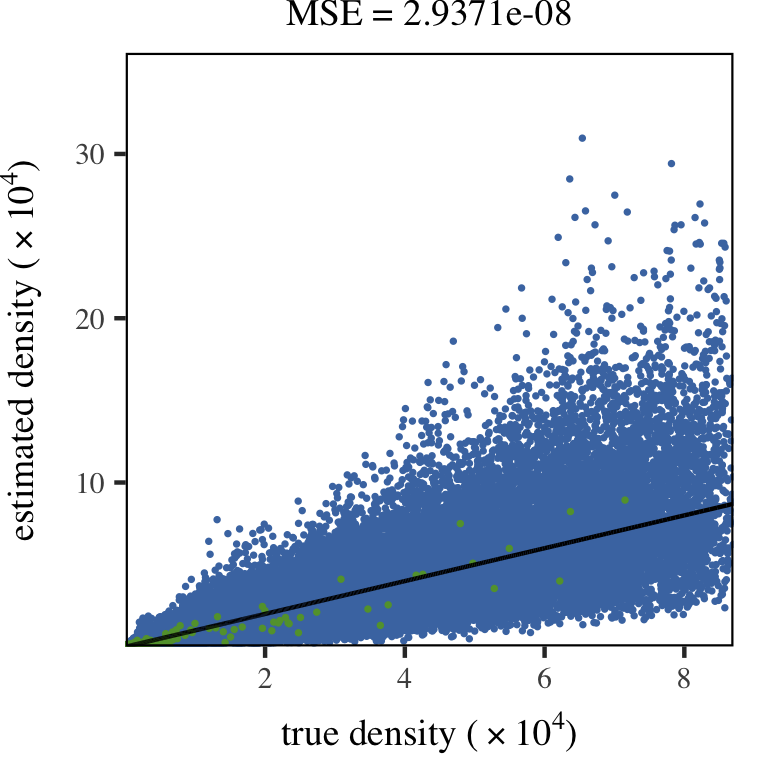
\includegraphics[keepaspectratio=true, width=\textwidth, height=0.23\textheight]{result/img/results_baakman_4_60000_mbe_silverman}
	\caption{Set \baakmanFour, \mbe}
	\label{fig:results:singlesphere:mbe:baakman4}
\end{subfigure}	
% Baakman 4 - SAMBE
\begin{subfigure}{0.3\textwidth}
	\centering
	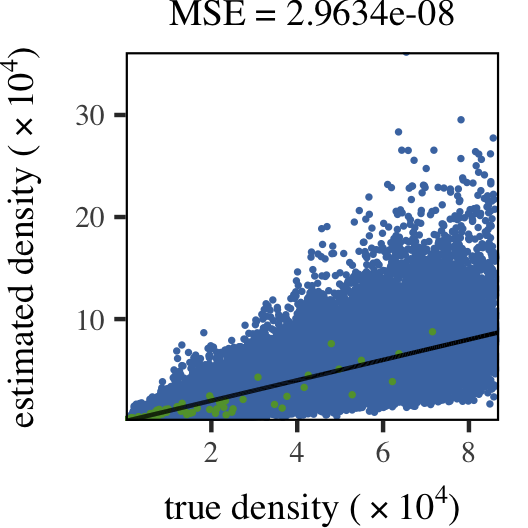
\includegraphics[keepaspectratio=true, width=\textwidth, height=0.23\textheight]{result/img/results_baakman_4_60000_sambe_silverman}
	\caption{Set \baakmanFour, \sambe}
	\label{fig:results:singlesphere:sambe:baakman4}
\end{subfigure}		
\subfigvspace
% Baakman 5 - MBE
\begin{subfigure}{0.3\textwidth}
	\centering
	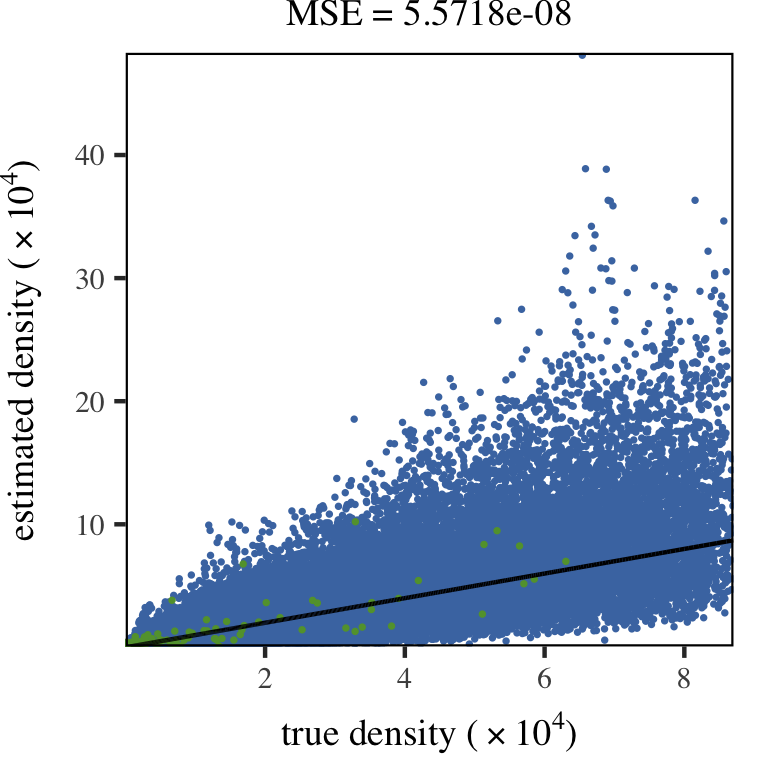
\includegraphics[keepaspectratio=true, width=\textwidth, height=0.23\textheight]{result/img/results_baakman_5_60000_mbe_silverman}
	\caption{Set \baakmanFive, \mbe}
	\label{fig:results:singlesphere:mbe:baakman5}
\end{subfigure}
% Baakman 5 - SAMBE
\begin{subfigure}{0.3\textwidth}
	\centering
	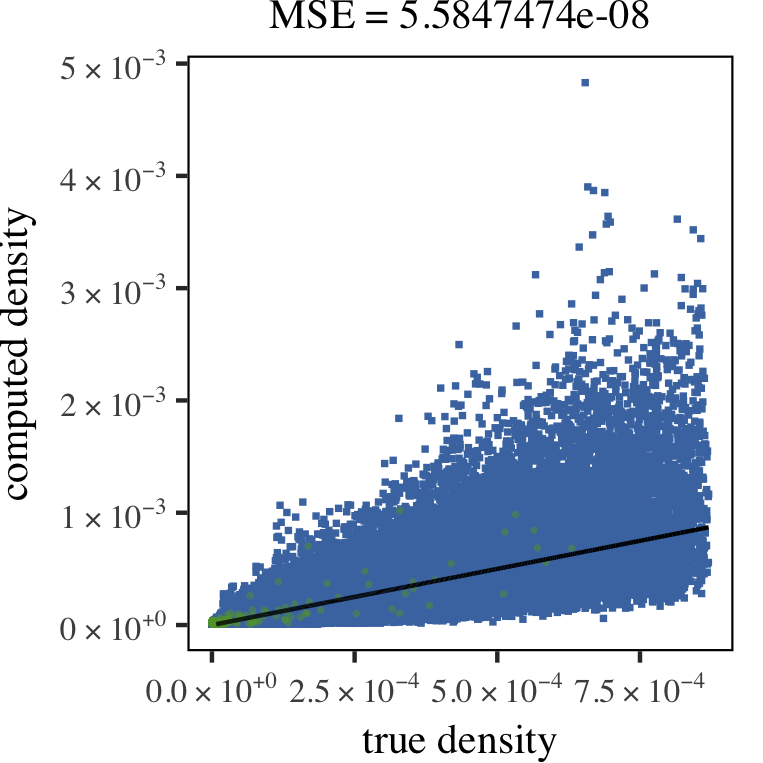
\includegraphics[keepaspectratio=true, width=\textwidth, height=0.23\textheight]{result/img/results_baakman_5_60000_sambe_silverman}
	\caption{Set \baakmanFive, \sambe}
	\label{fig:results:singlesphere:sambe:baakman5}
\end{subfigure}	
	\caption{Plot of the estimated density as a function of the known density of the datasets with a single Gaussian by (\subref{fig:results:singlesphere:mbe:ferdosi1}-\subref{fig:results:singlesphere:mbe:baakman5}) \mbe and (\subref{fig:results:singlesphere:sambe:ferdosi1}-\subref{fig:results:singlesphere:sambe:baakman5}) \sambe.}
	\label{fig:results:singleSphere:comparativePlots}
\end{figure*}

\begin{table}
	\centering
	%!TEX root = ../../paper.tex

\begin{tabular}{l*{2}{S[scientific-notation=true, round-mode=places,round-precision=3]}}
\toprule
~ 				& \multicolumn{2}{c}{Estimator}\\ \cmidrule{2-3}
Set				& {\mbe}					& {\sambe}	\\
\midrule
\ferdosiOne		& 8.30580618349064E-09		&  8.9087329457441E-09 \\
\baakmanOne		& 1.49022877061299E-08		&  1.5398737157543E-08 \\	
\baakmanFour	& 2.93709420107411E-08		&  2.9634323205557E-08 \\	
\baakmanFive	& 5.57179476550916E-08		&  5.5847473903432E-08 \\	
\bottomrule
\end{tabular}
	\caption{Performance of the Modified Breiman Estimator with fixed-shaped and shape-adaptive kernels on the datasets with a single Gaussian.} 	
	\label{tab:results:singleSphere:mse}
\end{table}

This section compares the performance of the Modified Breiman Estimator and a shape-adaptive variant on datasets that contain one Gaussian, \ie dataset \ferdosiOne, \baakmanOne, \baakmanFour, and \baakmanFive. Comparing the mean squared errors of the \mbe with those of \sambe in \cref{tab:results:singleSphere:mse} we find that the two estimators perform comparably, but that the fixed-shape estimator always gives a slightly lower mean squared error. This is confirmed by the visualization of the result in \cref{fig:results:singleSphere:comparativePlots} where hardly any difference is visible between \cref{fig:results:singlesphere:mbe:ferdosi1,fig:results:singlesphere:mbe:baakman1,fig:results:singlesphere:mbe:baakman4,fig:results:singlesphere:mbe:baakman5} and \cref{fig:results:singlesphere:sambe:ferdosi1,fig:results:singlesphere:sambe:baakman1,fig:results:singlesphere:sambe:baakman4,fig:results:singlesphere:sambe:baakman5}, respectively.

	% Ferdosi 1
		Comparing \cref{fig:results:singlesphere:mbe:ferdosi1} with \cref{fig:results:singlesphere:sambe:ferdosi1} we find hardly any difference between the results of the two estimators, \sambe overshoots some densities more than \mbe, but otherwise the results seem identical, which fits with the small difference in mean square error. 
		% Difference between components ?
		Reviewing the mean squared errors of the components of this dataset we find that \mbe slightly outperforms \sambe on both datasets.

	% Baakman 1
		\Cref{fig:results:singlesphere:mbe:baakman1,fig:results:singlesphere:sambe:baakman1} confirm what the MSE already told us, there is hardly any difference in performance between the two estimators. 
		% Difference between components ?
		There is no difference within the estimators between components. 

	% Baakman 4
		Based on the differences between \cref{fig:results:singlesphere:mbe:baakman4,fig:results:singlesphere:sambe:baakman4} we can at best conclude that the shape-adaptive estimator overestimates the densities slightly more than the fixed-shape estimator. 
		% Difference between noise and gaussian?
		The differences between estimators within components are not significantly large.

	% Baakman 5
		\Cref{fig:results:singlesphere:mbe:baakman5,fig:results:singlesphere:sambe:baakman5} supports the MSE in that there hardly any difference in estimated densities between the two estimators on dataset \baakmanFive. 
		% Difference between noise and gaussian?
		Furthermore within components the differences between the estimators are also negligible. 

	% Algehele observatie voor single sphere datsets
		\todo[inline]{General observation}
		\todo[inline]{What is the influence of elongatedness on the density estimate?}
		\todo[inline]{There is a difference within components, both estimators have a lower mse on the noise component than on the gaussian component.}
